\usepackage{comment}
\begin{comment}

Bilder/Graphiken implementieren:
-> Bildbreite auf Seitenbreite angepasst
-> [Inhalt] für Feintuning der Position
    h, here
    t, top
    b, bottom
    p, page of float
    htb, at the excact position

caption: Benennung unterhalb der Graphik
label: Referenz zur Verwendung im Text (Bsp: Wie in Abbildung \ref{fig:render} zu sehen...

\begin{figure}[htb]
    \centering  
    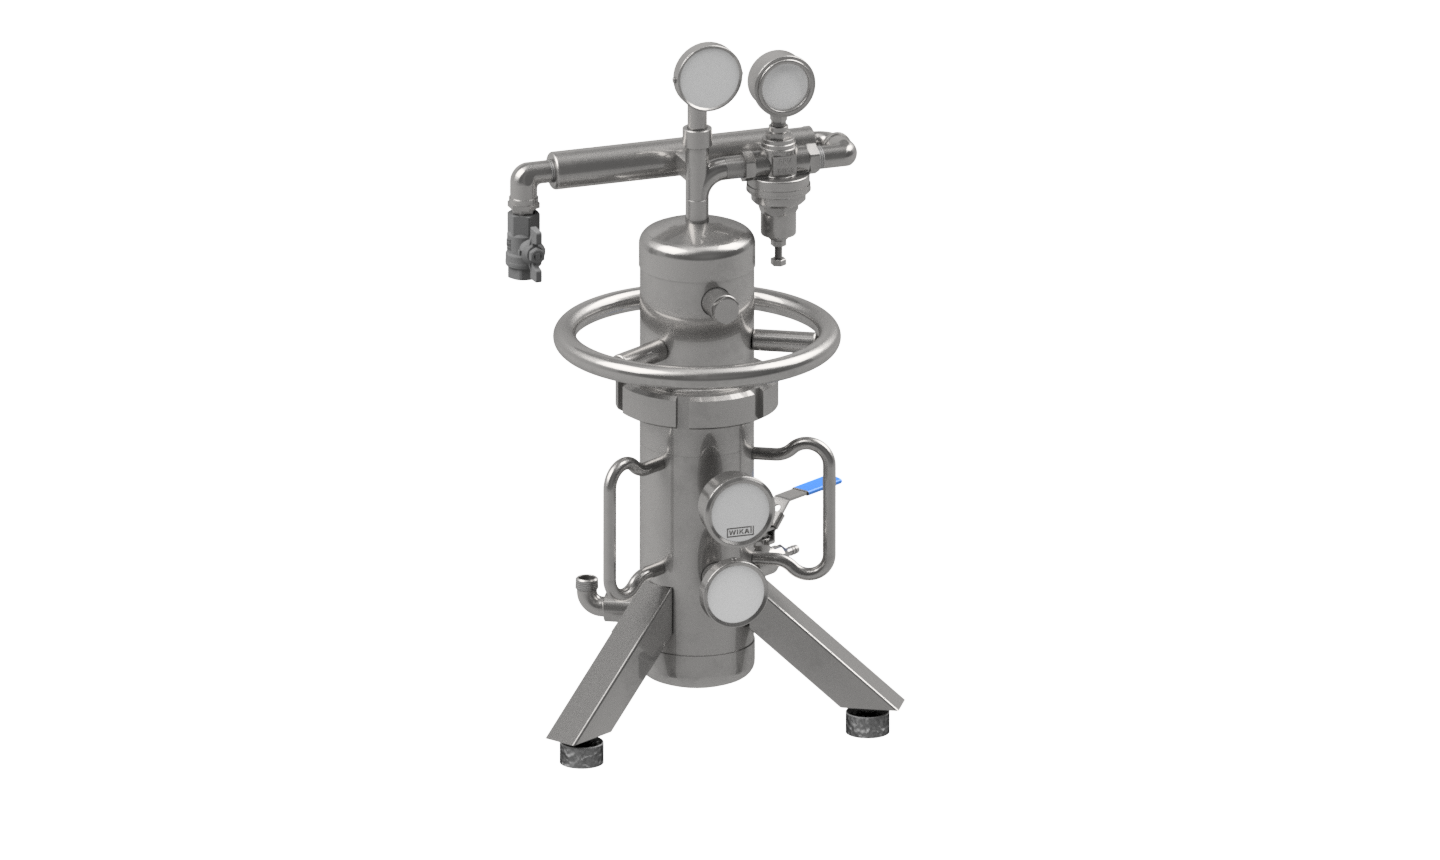
\includegraphics[keepaspectratio,width=\textwidth,height=\textheight]{render.png}
    \caption{3D Darstellung des Dampfdruckbehälters}\label{fig:render}
\end{figure}



Kapitel und Überschriften anlegen:
\section{Oberkapitel 1}
\subsection{Unterkapitel 1.1}
\section*{Oberkapitel 2} %Kapitel ohne Nummerierung


Zeilenumbrüche:
Hier entsteht ein neuer Zeilenbruch\newline
Hier auch.\\ %gleichwertig mit newline
 
Absätze:
Ein neuer Absatz\par                    %Abstand einmalig in der Präambel festgelegt
Ein individueller Absatz.\vfill{2cm}   
%Verschiedene Absätze mit {\bigskip, \smallskip\parskip} etc. 

Neue Seite: \newpage







\begin{center}
    Dieser Text steht zentriert.
\end{center}


%Tabellen erstellen, siehe 
%https://de.wikibooks.org/wiki/LaTeX-Kompendium:_Tabellen
%https://de.overleaf.com/learn/latex/Tables
%https://de.wikibooks.org/wiki/LaTeX-W%C3%B6rterbuch:_tabular

\begin{table}[h!]
\centering
\begin{tabular}{|c | c c|} 
 \hline
 Einheit & Benennung & Kategorie \\ %[0.5ex] 
 \hline
 m & 6 & 8783 \\ 
 s & 7 & 78 \\
 V & 545 & 778\\
 A & 545 & 18744\\
 \hline
\end{tabular}
\caption{Eine sehr vielaussagende Tabelle}      %Beschriftung unten und im Abbildungsverzeichnis
\label{wichtig}                                 %Referenz zum Verweis im Text mit \ref{tab:wichtig}
\end{table}


%Formeln und Gleichungen 
%https://de.overleaf.com/learn/latex/Mathematical_expressions
%https://www.namsu.de/Extra/pakete/amsmath/Amsmath.html
%Align Umgebung verwenden: (Equatation ist nicht so gut)
%
%    Verwenden Sie niemals leere Zeilen innerhalb der Gleichungsumgebungen.
%    Die letzte Zeile benötigt keinen Zeilenumbruch.
%

\begin{align}
\intertext{ Zum einen gilt: } 
a+b&=c
\intertext{zum anderen jedoch auch } 
b=c
\end{align}

%Formel ohne Nummer und Nachweis: 
\begin{align*}

    
\end{align*}




%\text bei Text in Formel:
\begin{align*}  
a - b &\geq 0 \text{ wenn } b \leq a \\  
\intertext{ andernfalls gilt }  
a -b &< 0  
\end{align*}




\end{comment}




